\begin{table*}[tbp]
\centering
\small
\renewcommand{\arraystretch}{1.2}
\begin{tabular}{p{1.23\columnwidth}|ccc}
\hline
\textbf{Question:} What is the difference between a mixed and pure culture & \multicolumn{3}{c}{\bf{Scores}}\\ \hline
\multicolumn{1}{l|}{\bf{Answer Candidates:}} & \bf{Boundary} & \bf{Content} & \bf{Verification} \\
\textbf{[1]} A culture is a society's total way of living and a society is a group \ldots & \ensuremath{\bf{1.0\times10^{-2}}} & \ensuremath{\bf{1.0\times10^{-1}}} & \ensuremath{1.1\times10^{-1}} \\
\textbf{[2]} The mixed economy is a balance between socialism and capitalism. & \ensuremath{1.0\times10^{-4}} & \ensuremath{4.0\times10^{-2}} & \ensuremath{3.2\times10^{-2}} \\
\textbf{[3]} A pure culture is one in which only one kind of microbial species is \ldots & \ensuremath{5.5\times10^{-3}} & \ensuremath{7.7\times10^{-2}} & \ensuremath{1.2\times10^{-1}} \\
\textbf{[4]} A pure culture comprises a single species or strains. A mixed  \ldots & \ensuremath{2.7\times10^{-3}} & \ensuremath{8.1\times10^{-2}} & \ensuremath{1.3\times10^{-1}} \\
\textbf{[5]} A pure culture is a culture consisting of only one strain. & \ensuremath{5.8\times10^{-4}} & \ensuremath{7.9\times10^{-2}} & \ensuremath{5.1\times10^{-2}} \\
\textbf{[6]} \textbf{A pure culture is one in which only one kind of microbial species  \ldots} & \ensuremath{5.8\times10^{-3}} & \ensuremath{9.1\times10^{-2}} & \ensuremath{\bf{2.7\times10^{-1}}} \\
\multicolumn{1}{c|}{\bf{\ldots \ldots}} & \multicolumn{3}{c}{\bf{\ldots \ldots}}\\ \hline                               
\end{tabular}
\caption{Scores predicted by our model for the answer candidates shown in \tabref{tab:example}. Although the candidate [1] gets high boundary and content scores, the correct answer [6] is preferred by the verification model and is chosen as the final answer.}
\label{tab:case-study}
\end{table*}

\section{Analysis and Discussion}
\label{analysis}



\subsection{Ablation Study}

%\begin{table}[htbp]
%\centering
%\begin{tabular}{|l|c|c|}
%\hline
%Model           & ROUGE-L & BLEU-1 \\ \hline
%Complete Model      & 45.65   &  43.97 \\
% - Answer Verification  &  44.38  & 43.76  \\
% - Content Model   & 44.27   & 44.17  \\
% - Joint Training  &         &          \\
% - YesNo Classification &  41.87  &  43.35 \\ 
%Boundary Baseline   &  38.95  &  42.52 \\ \hline
%\end{tabular}
%\caption{Ablation study on the development set of MS-MARCO}
%\label{tab:ablation}
%\end{table}




To get better insight into our system, we conduct in-depth ablation study on the development set of MS-MARCO, which is shown in \tabref{tab:ablation}. Following \newcite{snet}, we mainly focus on the ROUGE-L score that is averaged case by case. 

We first evaluate the answer verification by ablating the cross-passage verification model so that the verification loss and verification score will not be used during training and testing. Then we remove the content model in order to test the necessity of modeling the content of the answer. Since we don't have the content scores, we use the boundary probabilities instead to compute the answer representation for verification. Next, to show the benefits of joint training, we train the boundary model separately from the other two models. Finally, we remove the yes/no classification in order to show the real improvement of our end-to-end model compared with the baseline method that predicts the answer with only the boundary model. 

From \tabref{tab:ablation}, we can see that the answer verification makes a great contribution to the overall improvement, which confirms our hypothesis that cross-passage answer verification is useful for the multi-passage MRC. For the ablation of the content model, we analyze that it will not only affect the content score itself, but also violate the verification model since the content probabilities are necessary for the answer representation, which will be further analyzed in \secref{necessity}. Another discovery is that jointly training the three models can provide great benefits, which shows that the three tasks are actually closely related and can boost each other with shared representations at bottom layers. At last, comparing our method with the baseline, we achieve an improvement of nearly 3 points without the yes/no classification. This significant improvement proves the effectiveness of our approach.

\subsection{Case Study}

To demonstrate how each module of our model takes effect when predicting the final answer, we conduct a case study in \tabref{tab:case-study} with the same example that we discussed in \secref{introduction}. For each answer candidate, we list three scores predicted by the boundary model, content model and verification model respectively. 

On the one hand, we can see that these three scores generally have some relevance. For example, the second candidate is given lowest scores by all the three models. We analyze that this is because the models share the same encoding and matching layers at bottom level and this relevance guarantees that the content and verification models will not violate the boundary model too much. On the other hand, we also see that the verification score can really make a difference here when the boundary model makes an incorrect decision among the confusing answer candidates ([1], [3], [4], [6]). Besides, as we expected, the verification model tends to give higher scores for those answers that have semantic commonality with each other ([3], [4], [6]), which are all valid answers in this case. By multiplying the three scores, our model finally predicts the answer correctly.  

% \subsection{How does the Content Model Work ?}
\subsection{Necessity of the Content Model}
\label{necessity}
\begin{figure*}[tb]
\centering
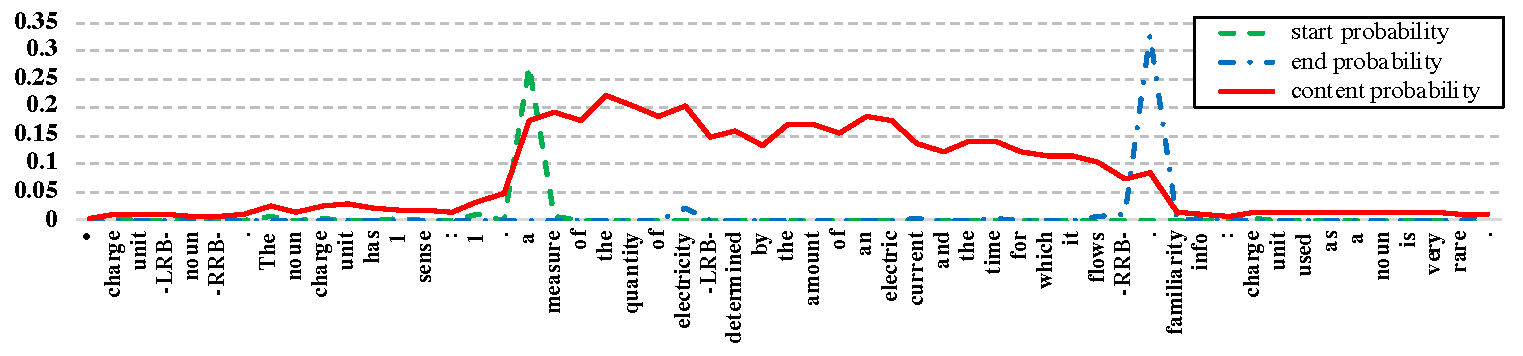
\includegraphics[width=\textwidth]{score.pdf}

\caption{The boundary probabilities and content probabilities for the words in a passage}
\label{fig:content}
\end{figure*}

% In our model, we compute the answer representation based on the content probabilities predicted by a separate content module instead of directly using the boundary probabilities. We argue that modeling answers semantic meaning is necessary if we want the content based verification really takes effects. \figref{fig:content} plots the predicted content probabilities as well as the boundary probabilities for a passage. We can see that the boundary and content probabilities capture different factors of the answer. Since answer candidates usually have similar boundary words, it is difficult for boundary models to capture the differences among the answer candidates, which ability is important for verification. On the contrary, by using the content probabilities, we are able to pay more attention to the content part of the answer, which could be different for different answer candidates and able to support cross-passage verification. Furthermore, the content probabilities could also adjust the weights of the words so that unimportant words (e.g. ``and'' and ``.'') within the answer span and enable verification to focused on important words. We believe that this refined representation is good for the answer verification process.

In our model, we compute the answer representation based on the content probabilities predicted by a separate content model instead of directly using the boundary probabilities. 
% As is shown in the ablation study, the content model is important for the overall improvement. 
We argue that this content model is necessary for our answer verification process.  \figref{fig:content} plots the predicted content probabilities as well as the boundary probabilities for a passage. We can see that the boundary and content probabilities capture different aspects of the answer. 
Since answer candidates usually have similar boundary words, if we compute the answer representation based on the boundary probabilities, it's difficult to model the real difference among different answer candidates.
% If we compute the answer representation based on the boundary probabilities, it's difficult to capture the differences among the answer candidates since those candidates usually have similar words near the boundary. 
On the contrary, with the content probabilities, we pay more attention to the content part of the answer, which can provide more distinguishable information for verifying the correct answer. Furthermore, the content probabilities can also adjust the weights of the words within the answer span so that unimportant words (e.g. ``and'' and ``.'') get lower weights in the final answer representation. We believe that this refined representation is also good for the answer verification process.


% Actually, it is natural to pay attention to the answer content when our humans answer questions. However, for reading comprehension model, directly predicting whether each word should be included in the content is not an effective way to extract a valid answer since the predicted content words may be discontinuous pieces. Therefore, we propose to predict the content jointly with the boundary model. This make it possible to still employ the boundary model for extracting answer spans while the content scores can be used to measure whether each candidate is good or not. \figref{fig:content} shows the the predicted content probabilities as well as the boundary probabilities for a passage. We can see that the boundary and content probabilities reflects different aspects of the answer. Therefore, we average the content scores of all the words in an answer to measure the content quality.

% Another important function of content model is to compute the answer representation based on the predicted content probabilities. We can see that the predicted content probabilities can really capture the important words in the passage, which usually accords with the answer boundary. Furthermore, the content probabilities could adjust the weights of the words so that unimportant words (e.g. ``and'' and ``.'') within the answer span also get lower weights in the final answer representation. We believe that this refined representation is good for the answer verification process.
%From our point of view, our method to model the content has three benefits.
%First, we can still use the effective boundary model to extract candidate spans from passages while the content score can be used to measure whether each candidate is good or not, and will play a factor in the final decision. 
%Second, the content scores usually accord with the the span predicted by boundary model. Therefore, we can calculate the answer representation based on the content scores.
%Third, the content loss can serve as a correction term to the boundary loss. As is pointed out in \newcite{dcn+}, only using the boundary loss encourages exact answers at the cost of penalizing overlapping answers. By taking the content into consideration, overlapping answers will get less penalization than totally unmatched answers. Furthermore, our loss function is differentiable, compared with the reinforced approach in \newcite{dcn+}.
%   


